\documentclass[aspectratio=169]{beamer}

\usetheme{default}

\usepackage[utf8]{inputenc}
\usepackage[russian]{babel}
\usepackage[OT1]{fontenc}
\usepackage{amsmath}
\usepackage{amsfonts}
\usepackage{amssymb}
\usepackage{graphicx}
\usepackage{etoolbox}
\usepackage{caption}
\usepackage{subcaption}
\captionsetup{compatibility=false}
\usepackage{pifont}
%\usepackage{subfigure}
\usepackage{xcolor}
\usepackage{framed}
\usepackage{empheq}
\usepackage[many]{tcolorbox}
\usepackage{multirow}
\usepackage{tikz}
\usepackage{listings}
\usepackage{tikz}

\definecolor{shadecolor}{cmyk}{0,0,0,1}

\lstset{
	backgroundcolor=\color{lightgray},
	commentstyle=\color{blue},
	frame=single
	breakatwhitespace,
	language=python,
	columns=fullflexible,
	keepspaces,
	breaklines,
	tabsize=3,
	showstringspaces=false,
	extendedchars=true,
	numbers=left
}

\makeatletter

\setbeamercolor{title}{fg=white}
\setbeamercolor{frametitle}{fg=black}
\setbeamerfont*{title}{family=\sffamily,size=\LARGE}

\setbeamerfont{page number in head/foot}{size=\scriptsize}
\setbeamertemplate{footline}[frame number]
\let\otp\titlepage
\renewcommand{\titlepage}{\otp\addtocounter{framenumber}{-1}}

\setbeamertemplate{background canvas}{%
	\ifnumequal{\c@framenumber}{0}{%
		\vbox to \paperheight{\vfil\hbox to \paperwidth{\hfil
\includegraphics[height=\paperheight]{images/cover.png}\hfil}\vfil}
   }{%
      \ifnumequal{\c@framenumber}{\inserttotalframenumber}{
        \vbox to \paperheight{\vfil\hbox to \paperwidth{\hfil
\includegraphics[height=\paperheight]{images/back.png}\hfil}\vfil}
      }{%
         % Other frames
      }%
   }%
}

\makeatother

\beamertemplatenavigationsymbolsempty

\tcbset{highlight math style={enhanced,colframe=red,colback=white,arc=4pt,boxrule=1pt}}

\usetikzlibrary{shadings,shadows,shapes.arrows}

\newcommand*{\tikzarrow}[2]{%
  \tikz[
    baseline=(A.base),             % Set baseline to the baseline of node content
    font=\footnotesize\sffamily    % Set fontsize of the node content
  ]
  \node[
    single arrow,                  % Shape of the node
    single arrow head extend=5pt,  % Actual width of arrow head
    draw,                          % Draw the node shape
    inner sep=3pt,                 % Separation between node content and node shape
    top color=#1,               % Shading color on top of node
    bottom color=#1,               % Shading color on bottom of node
    % drop shadow                    % Draw a shadow
  ] (A) {#2};%
}

\newcommand{\tikzfancyarrow}[2][2cm]{\tikz[baseline=-0.5ex]\node [arrowstyle=#1] {#2};}
\newcommand*\rot{\rotatebox{90}}

\author{Стройкова Ксения}
\title{\newline \newline \newline Лекция 4 \\ Различные аспекты кластеризации}

\begin{document}

\begin{frame}[plain]
\titlepage
\end{frame}

\begin{frame}{Краткое содержание предыдущих лекций}

\vspace{1em}
{\bf Дано.} Признаковые описания $N$ объектов $\mathbf{x} = (x_1, \ldots, x_m) \in \mathcal{X}$, образующие тренировочный набор данных $X$

\vspace{1em}
{\bf Найти.} Модель из семейства параметрических функций
\[
H = \{h(\mathbf{x, \mathbf{\theta}}): \mathcal{X} \times \Theta \rightarrow \mathcal{Y} \mid \mathcal{Y} = \{1, \ldots, K\}\},
\]
ставящую в соответствие произвольному $\mathbf{x} \in \mathcal{X}$ один из $K$ кластеров так, чтобы объекты внутри одного кластера были похожи, а объекты из разных кластеров различались

\end{frame}

\begin{frame}{Краткое содержание предыдущих лекций}

\begin{columns}[]
    \begin{column}{.4\textwidth}
    	Рассмотрели классические алгоритмы кластеризации
		\begin{enumerate}
					\item Hierarchical Clustering
			\item dbscan, OPTICS
			\item Смесь гауссовских распределений и k-means
		\end{enumerate}

    \end{column}

    \begin{column}{.6\textwidth}
    \vspace{-0em}
	\begin{center}
   		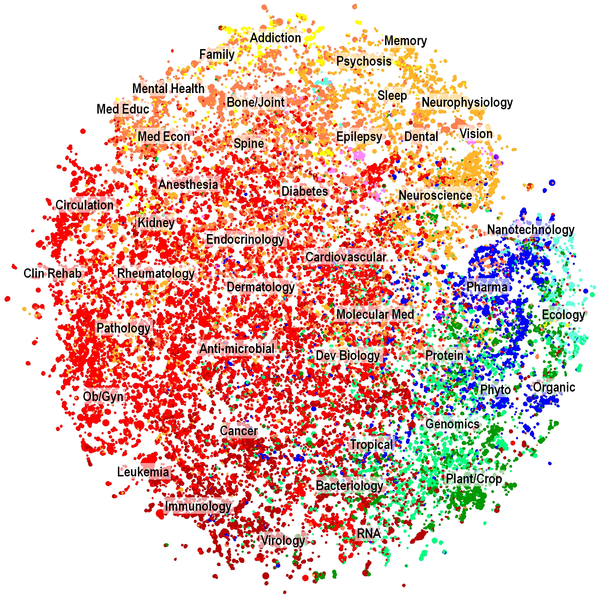
\includegraphics[width=\textwidth]{images/medical.png}
    \end{center}
    \end{column}
  \end{columns}

\end{frame}

% ============================================== %

\section{Байесовская кластеризация + EM}

% ============================================== %

\begin{frame}

\begin{center}
{\Large Байесовская кластеризация + EM}

\vspace{1em}
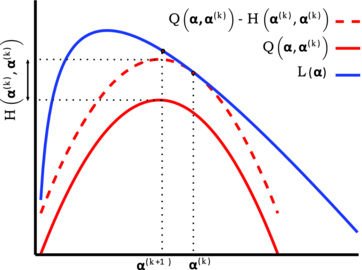
\includegraphics[height=0.5\textheight]{images/em.jpg}
\end{center}

\end{frame}

\begin{frame}{Expectation Maximization}

{\bf Дано.} \\ Известно распределение $P(\mathbf{X}, \mathbf{Z} | \theta)$, где $\mathbf{x}$ -- наблюдаемые переменные, а $\mathbf{z}$ -- скрытые.

{\bf Найти.} \\ $\theta$,  максимизирующее $P(\mathbf{X} | \theta)$.

\vspace{1em}
\begin{itemize}
\item[E] вычислить $P(\mathbf{Z} | \mathbf{X}, \theta^{old})$ при фиксированном $\theta^{old}$
\item[M] вычислить $\theta^{new} = \arg \max_{\theta} \mathcal{Q} (\theta, \theta^{old})$, где
\[
\mathcal{Q} (\theta, \theta^{old}) = E_\mathbf{Z}[\ln p(\mathbf{X}, \mathbf{Z} | \theta)] = \sum_{\mathbf{Z}} p(\mathbf{Z} | \mathbf{X}, \theta^{old}) \ln p(\mathbf{X}, \mathbf{Z} | \theta))
\]
\end{itemize}

\end{frame}

\begin{frame}{Кластеризация пользователей стримингового сервиса}

\begin{columns}[T]
    \begin{column}{.5\textwidth}
    \begin{center}
   		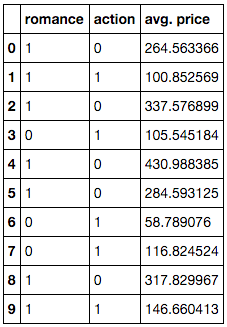
\includegraphics[scale=0.5]{images/movies_data.png}
    \end{center}
    \end{column}

    \begin{column}{.5\textwidth}
	Для каждого пользователя известно, есть ли у него/нее интерес к романтике, экшену и средняя цена купленных фильмов
    \end{column}
  \end{columns}

\end{frame}

\begin{frame}{}

\begin{center}
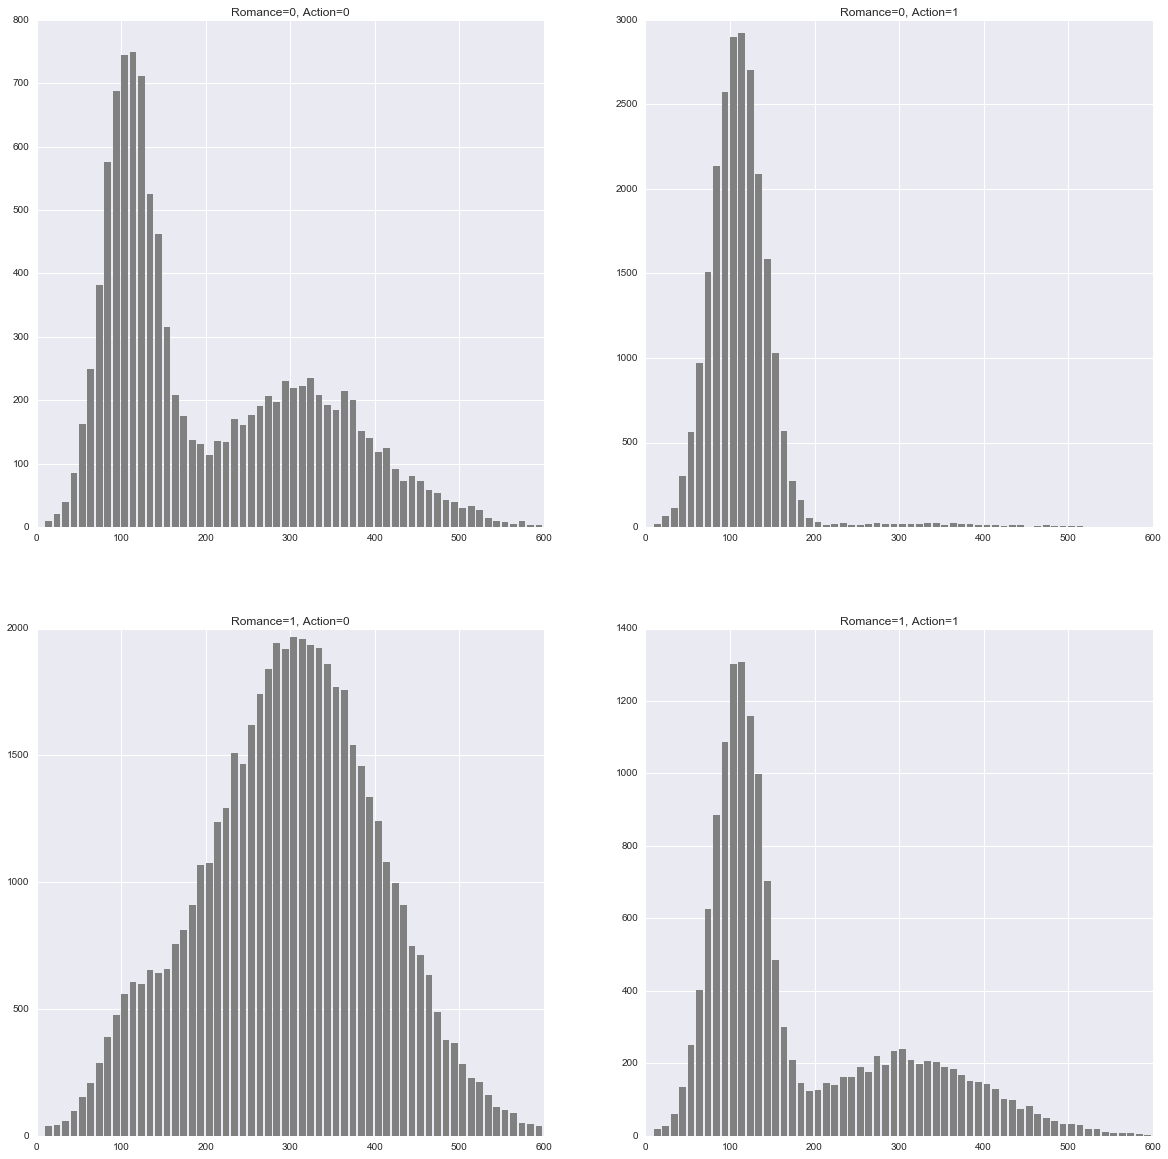
\includegraphics[height=0.8\textheight]{images/movies.png}
\end{center}

\end{frame}

\begin{frame}{Предположения модели}

Априорное распределение
\[
p(C_k) = \pi_k
\]
Распределение интересов
\[
p(I_i | C_k) \sim Ber(P_{ki})
\]
Распределение средней цены фильма
\[
p(x | C_k) \sim \mathcal{N}(x | \mu_k, \sigma_k)
\]

\end{frame}

\begin{frame}{Итерации EM}

\begin{itemize}
\item[E]
\[
\gamma_{nk} = p(z_n = k | u_n, \pi, P, \mu, \sigma) = \frac{\pi_k \mathcal{N}(x_n | \mu_k, \sigma_k) \prod_{i=1}^2 P_{ki}^{I_{ni}}(1 - P_{ki})^{1 - I_{ni}}}{\sum_j \pi_j \mathcal{N}(x_n | \mu_j, \sigma_j) \prod_{i=1}^2 P_{ji}^{I_{ni}}(1 - P_{ji})^{1 - I_{ni}}}
\]
\item[M]
\[
N_k = \sum_{n=1}^N \gamma_{nk}, \qquad \pi_k = \frac{N_k}{N}
\]
\[
P_{ki} = \frac{1}{N_k} \sum_{n=1}^N \gamma_{nk} I_{ni}, \quad \mu_{k} = \frac{1}{N_k} \sum_{n=1}^N \gamma_{nk} x_n, \quad \sigma_k = \frac 1 {N_k} \sum_{n=1}^N \gamma_{nk} ({x}_n - \mu_k)^2
\]
\end{itemize}

\end{frame}

\begin{frame}{}

\begin{center}
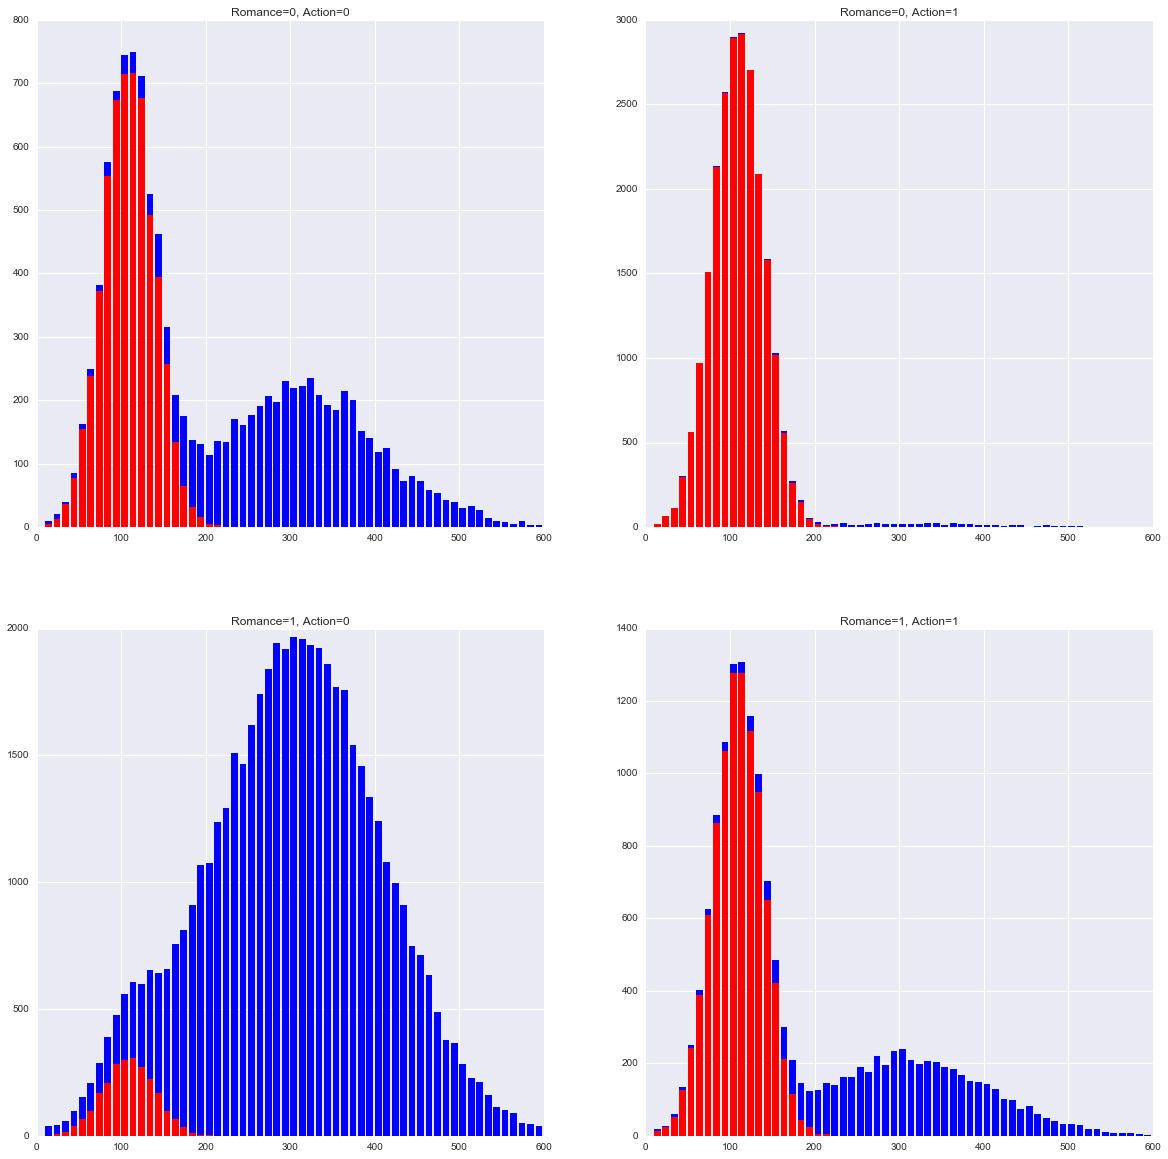
\includegraphics[height=0.8\textheight]{images/movies_res.png}
\end{center}

\end{frame}

% ============================================== %

\section{Функции расстояния}

% ============================================== %

\begin{frame}

\begin{center}
{\Large Функции расстояния}

\vspace{1em}
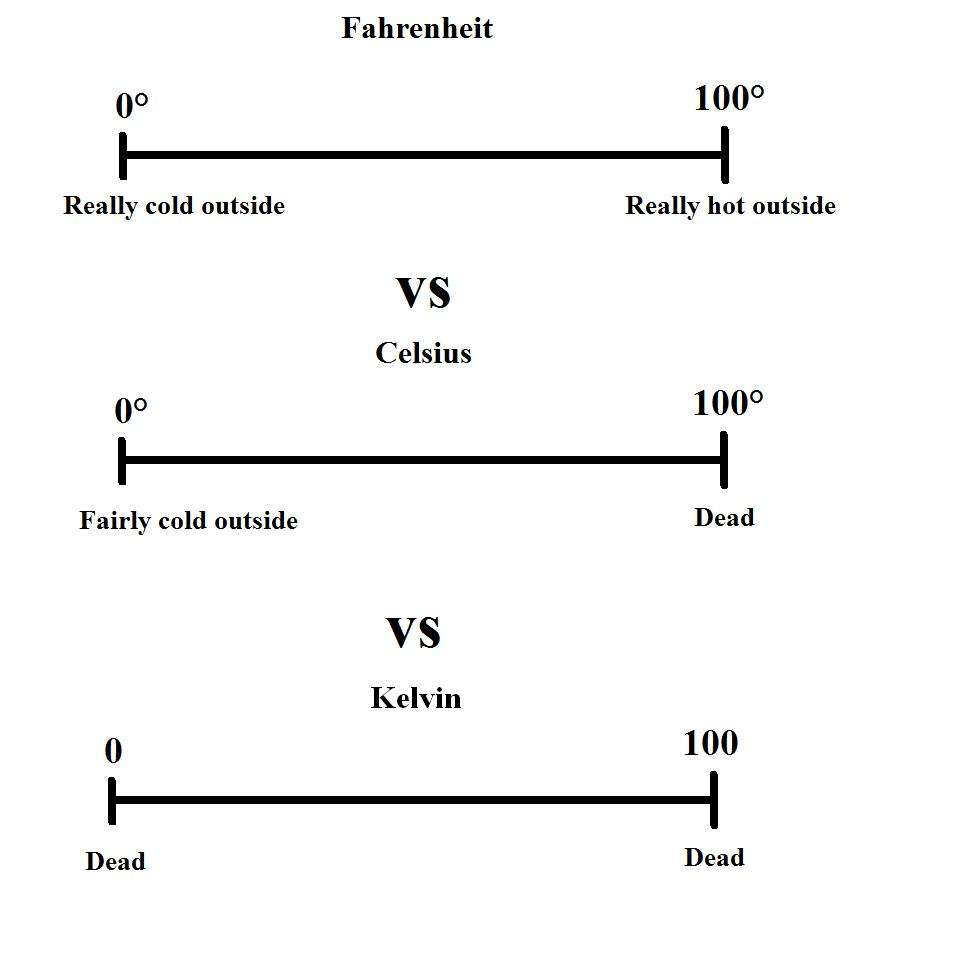
\includegraphics[height=0.8\textheight]{images/celsius.jpg}
\end{center}

\end{frame}

\begin{frame}{Модификации алгоритма}

Взять уже известную нам функцию потерь (инерцию) и ``поиграть'' с функцией расстояния.
\[
\tilde J(\mu) = \sum_{n=1}^N \sum_{k=1}^K r_{nk} d(\mathbf{x}_n, \mu_k), \quad r_{nk} = \begin{cases}
1, \; \text{для } k = \arg \min_j d(\mathbf{x}_n, \mu_j) \\
0, \; \text{иначе}
\end{cases}
\]
\end{frame}

\begin{frame}{Расстояния 1}

\begin{columns}[T]
    \begin{column}{.5\textwidth}
    \begin{itemize}
		\item Минковского
		\[
		d_r(\mathbf{x}, \mathbf{y}) = \left[ \sum_{j=1}^N |x_j - y_j|^r \right]^{\frac{1}{r}}
		\]
		\item Евклидово $r = 2$
		\[
		d_E(\mathbf{x}, \mathbf{y}) = d_2(\mathbf{x}, \mathbf{y})
		\]
		\item Манхэттэн $r = 1$
		\[
		d_M(\mathbf{x}, \mathbf{y}) = d_1(\mathbf{x}, \mathbf{y})
		\]
		\item $r=\infty$
		\[
		d_\infty(\mathbf{x}, \mathbf{y}) = \max_j |x_j - y_j|
		\]
	\end{itemize}
    \end{column}

    \begin{column}{.5\textwidth}
    \vspace{2em}
	\begin{center}
   		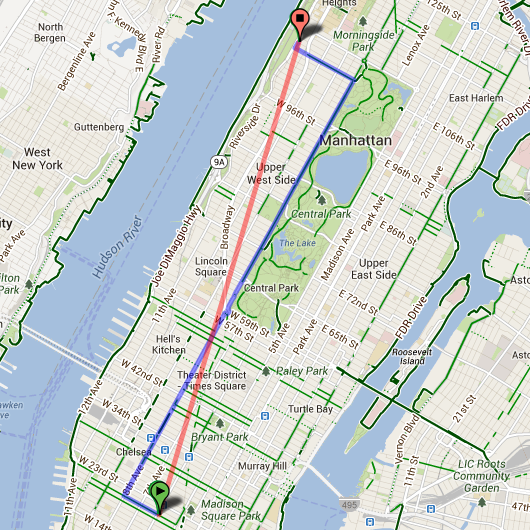
\includegraphics[scale=0.25]{images/manhattan.png}
    \end{center}
    \end{column}
  \end{columns}

\end{frame}

\begin{frame}

\begin{enumerate}
\item Функции расстояния чувствительны к ``масштабу'' данных
\begin{itemize}
\item Преобразовать обучающую выборку так, чтобы  признаки имели нулевое среднее и единичную дисперсию (standartization)
\item Преобразовать обучающую выборку так, чтобы значения признаков лежали на отрезке $[0, 1]$ (normalization)
\end{itemize}
\begin{center}
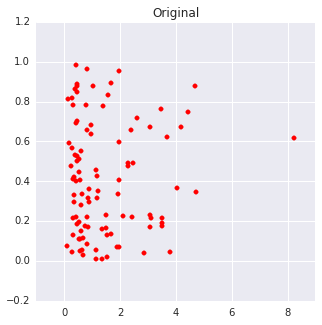
\includegraphics[scale=0.2]{images/orig.png}
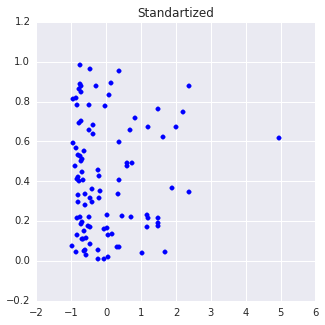
\includegraphics[scale=0.2]{images/std.png}
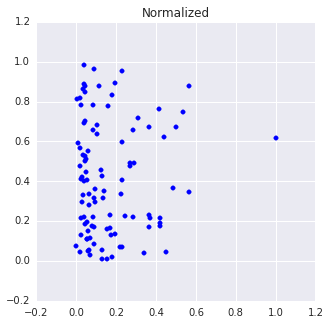
\includegraphics[scale=0.2]{images/norm.png}
\end{center}
\item Есть шанс улучшить качество, применив монотонное преобразование ($\log$, $\sqrt{\;}$)
\begin{center}
$  $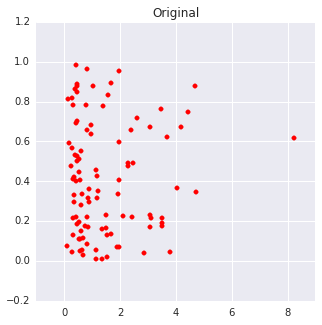
\includegraphics[scale=0.2]{images/orig.png}
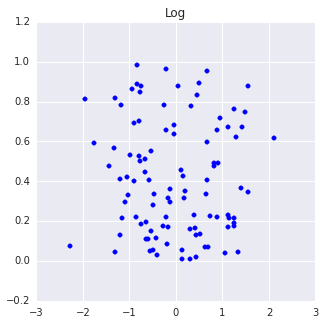
\includegraphics[scale=0.2]{images/log.png}
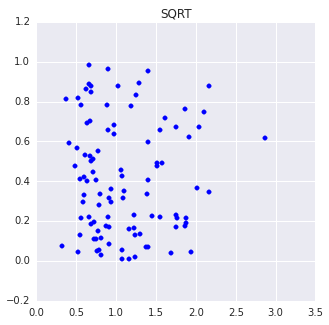
\includegraphics[scale=0.2]{images/sqrt.png}
\end{center}
\end{enumerate}

\end{frame}

\begin{frame}{Расстояния 2}

\begin{columns}[T]

    \begin{column}{.4\textwidth}
    \vspace{5em}
	\begin{center}
   		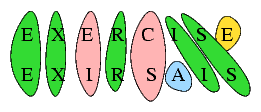
\includegraphics[scale=0.5]{images/edit.png}
    \end{center}
    \end{column}

    \begin{column}{.6\textwidth}
    \begin{itemize}
		\item Жаккар
		\[
		d_J(\mathbf{x}, \mathbf{y}) = 1 - \frac{|\mathbf{x} \cap \mathbf{y}|}{|\mathbf{x} \cup \mathbf{y}|}
		\]
		\item Косинус
		\[
		d_c(\mathbf{x}, \mathbf{y}) = \arccos \frac{\mathbf{x} \mathbf{y}}{\|\mathbf{x}\| \|\mathbf{y}\|}
		\]
		\item Правки \\
		{\it $d_e$ -- наименьшее количество удалений и вставок, приводящее $\mathbf{x}$ к $\mathbf{y}$.}
		\item Хэмминг \\
		{\it $d_H$ -- количество различных компонент в $\mathbf{x}$ и $\mathbf{y}$.}
	\end{itemize}

    \end{column}
  \end{columns}

\end{frame}

% ============================================== %

\section{Выбор количества кластеров}

% ============================================== %

\begin{frame}

\begin{center}
{\Large Выбор количества кластеров}

\vspace{2em}
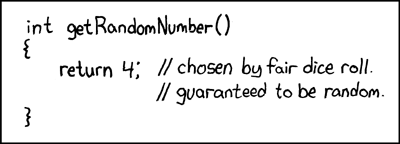
\includegraphics[width=0.7\textwidth]{images/random_number.png}
\end{center}

\end{frame}

\begin{frame}{Выбор наилучшего $K$}

{\it Идея.} Выбрать критерий качества кластеризации и построить его значение для $K = 1, 2, \ldots$

\begin{columns}[]
    \begin{column}{.5\textwidth}
    \begin{itemize}
	\item средняя сумма квадратов расстояния до центроида
	\item средний диаметр кластера
	\end{itemize}
    \end{column}
    \begin{column}{.5\textwidth}
    \vspace{1em}
    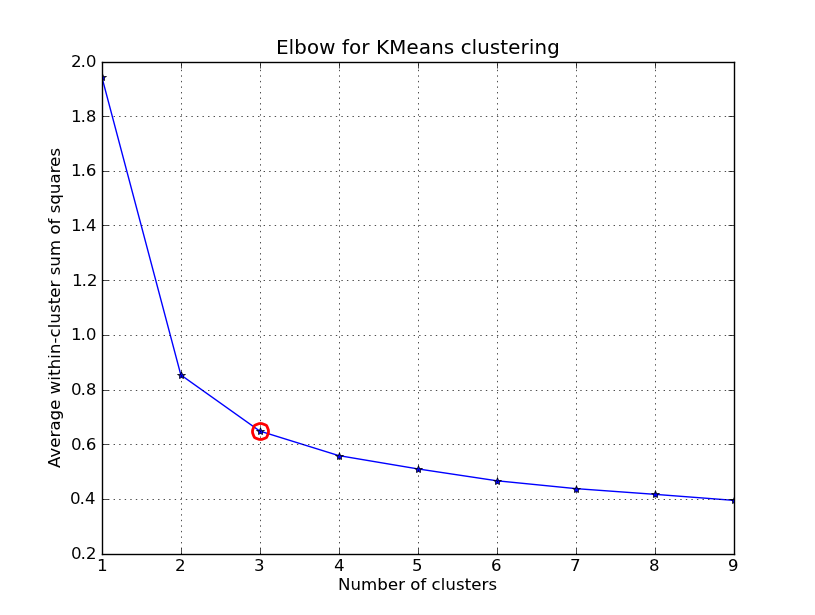
\includegraphics[scale=0.3]{images/elbow.png}
    \end{column}
\end{columns}

\end{frame}

\begin{frame}{Критерий Silhouette}

Пусть дана кластеризация в $K$ кластеров, и объект $i$ попал в $C_k$

\vspace{1em}
\begin{itemize}
\item $a(i)$ -- среднее расстояние от $i$ объекта до объектов из $C_k$
\item $b(i) = min_{j \neq k} b_j(i)$,  где $b_j(i)$ -- среднее расстояние от $i$ объекта до объектов из $C_j$
\end{itemize}
\[
silhouette(i) = \frac{b(i) - a(i)}{\max(a(i), b(i))}
\]
Средний silhouette для всех точек из $\mathbf{X}$ является критерием качества кластеризации.

\end{frame}

% ============================================== %

\section{Качество кластеризации}

% ============================================== %

\begin{frame}

\begin{center}
{\Large Качество кластеризации}


\includegraphics[scale=0.3]{images/quality.jpg}
\end{center}

\end{frame}

\begin{frame}{Качество кластеризации\footnote{\href{http://scikit-learn.org/stable/modules/clustering.html\#clustering-evaluation}{scikit-learn docs}}}

Пусть дана обучающая выборка, для которой правильная кластеризация $C$ известна. С помощью выбранного алгоритма получена кластеризация $K$. Проверить, насколько $K$ совпадает с $C$.

\vspace{1em}
\begin{itemize}
\item Adjusted Rand Index \\
{\it \small
$a$ -- кол-во пар объектов, попавших в один кластер и в $C$, и в $K$ \\
$b$ -- кол-во пар объектов, попавших в разные кластеры и в $C$, и в $K$
\[
RI = \frac{a+b}{C^N_2}, \quad ARI = \frac{RI - E_{rdm}[RI]}{\max(RI) - E_{rdm}[RI]}
\]
}
\item Mutual Information \\
{\it \small
\[
MI = \sum_{c \in C} \sum_{k \in K} p(c, k) \log \frac{p(c, k)}{p(k)p(c)}
\]
}
\end{itemize}

\end{frame}

% ============================================== %

\section{Multidimensional Scaling}

% ============================================== %

\begin{frame}

\begin{center}
{\Large Multidimensional Scaling}

\vspace{1em}

\includegraphics[width=0.8\textwidth]{images/curse.png}
\end{center}

\end{frame}

\begin{frame}{Идея метода}

Перейти в пространство меньшей размерности так, чтобы расстояния между объектами в новом пространстве были подобны расстояниям в исходном пространстве.

\end{frame}

\begin{frame}{t-Stochastic Neighbour Embedding (t-SNE)\footnote{\url{http://lvdmaaten.github.io/tsne/}}}

Схожесть между объектами в исходном пространстве
\[
p(i, j) = \frac{p(i | j) + p(j | i)}{2n}, \quad p(j | i) = \frac{\exp(-\|\mathbf{x}_j-\mathbf{x}_i\|^2/{2 \sigma_i^2})}{\sum_{k \neq i}\exp(-\|\mathbf{x}_k-\mathbf{x}_i\|^2/{2 \sigma_i^2})}
\]
Схожесть между объектами в целевом пространстве
\[
q(i, j) = \frac{(1 + \| \mathbf{y}_i - \mathbf{y}_j \|^2)^{-1}}{\sum_{k \neq l}(1 + \| \mathbf{y}_k - \mathbf{y}_l \|^2)^{-1}}
\]
Критерий
\[
J_{t-SNE} = KL(P \| Q) = \sum_i \sum_j p(i, j) \log \frac{p(i, j)}{q(i, j)} \rightarrow \min
\]

\end{frame}

\begin{frame}{t-распределение}

\[
\tau(\mu, \sigma^2, \nu) \propto \left[1 + \frac{1}{\nu}\left(\frac{x-\mu}{\sigma}\right)^2\right]^{-\frac{\nu+1}{2}}
\]

\begin{center}
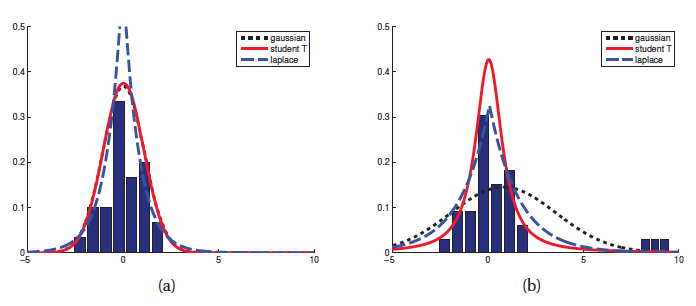
\includegraphics[scale=0.4]{images/t-distr.png}
\end{center}

Уильям Госсет 1908 (Student)

\end{frame}

\begin{frame}{Дивергенция Кульбака-Лейблера\footnote{\href{http://colah.github.io/posts/2015-09-Visual-Information/}{Visual Information Theory}}}

Насколько распределение $P$ отличается от распределения $Q$?
\[
KL(P \| Q) = \sum_z P(z) \log \frac{P(z)}{Q(z)}
\]

\end{frame}

\begin{frame}{Digits Dataset}

около 1800 картинок 8x8 с рукописными цифрами

\begin{center}
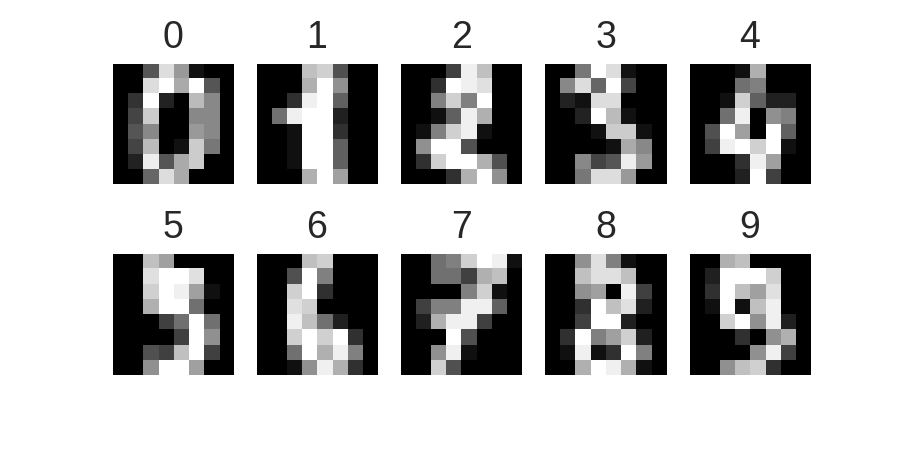
\includegraphics[scale=0.5]{images/digits.png}
\end{center}

\href{https://raw.githubusercontent.com/oreillymedia/t-SNE-tutorial/master/images/animation.gif}{t-SNE}

\end{frame}

\begin{frame}{MNIST Dataset}

70000 картинок 20x20 с рукописными цифрами

\begin{center}
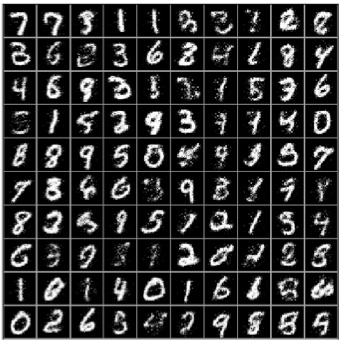
\includegraphics[scale=1.0]{images/mnistdigits.jpg}
\end{center}

\href{http://lvdmaaten.github.io/tsne/examples/mnist_tsne.jpg}{t-SNE}

\end{frame}

\begin{frame}{Еще примеры}

\href{http://lvdmaaten.github.io/tsne/examples/caltech101_tsne.jpg}{CalTech}

\vspace{1em}
\href{http://lvdmaaten.github.io/tsne/examples/SP500_tsne.png}{S\&P 500}

\vspace{1em}
\href{http://www.cs.toronto.edu/~hinton/turian.png}{Words}

\end{frame}

\begin{frame}{Еще алгоритмы}

\begin{center}
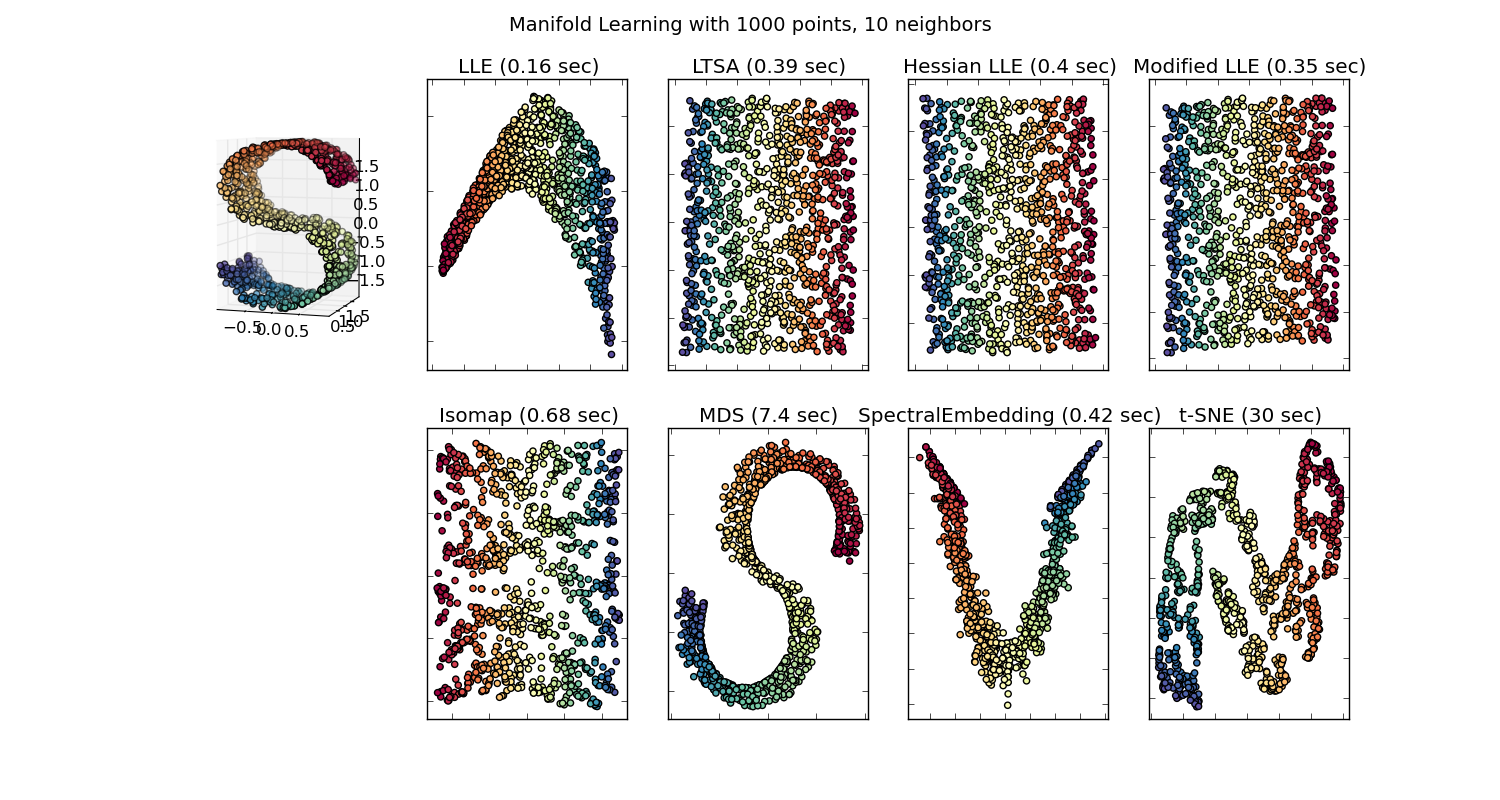
\includegraphics[scale=0.27]{images/mainfold.png}
\end{center}

\end{frame}

\begin{frame}[plain]
\begin{center}
{\Large Вопросы}
\end{center}
\end{frame}

\end{document}
